%!TEX root = report.tex

\appendix
\chapter{System Usability Scale} {
\label{app:system_usability_scale}

	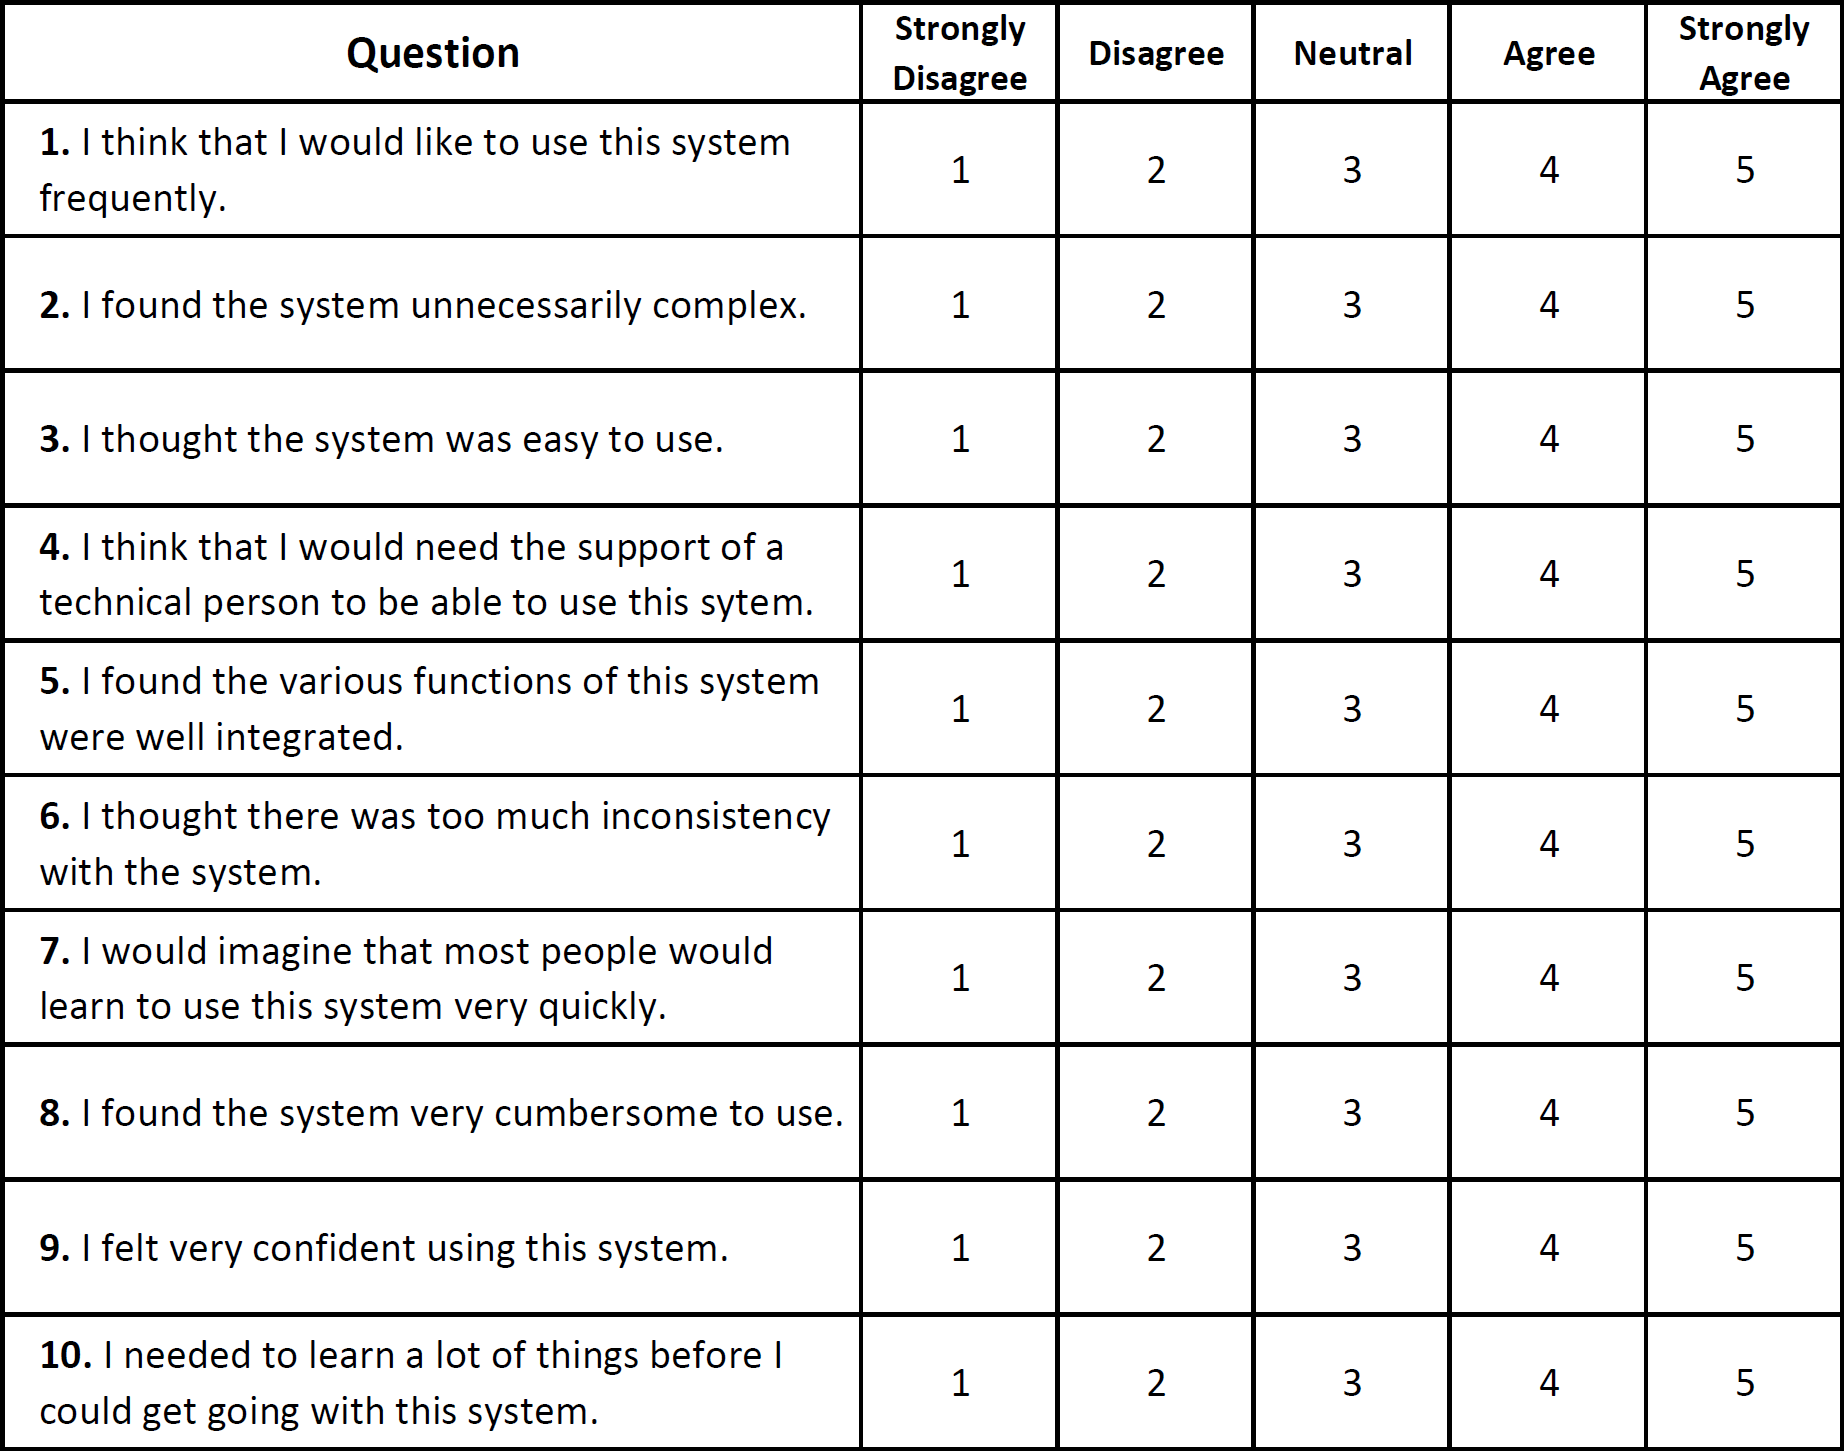
\includegraphics[width=\textwidth]{images/design/sus}

	The System Usability Scale (SUS) score is calculated by first converting each participant's score for each question to a new value. The values are obtained by performing $value - 1$ for each odd question and $5 - value$ for each even question. These values for each participant are then added together and multiplied by 2.5 to convert the original score from 0-40 to 0-100. Further, the SUS score should be considered in terms of percentile ranking instead of percentages.

	% \section{Questionnaire} {
	% \label{sec:questionnaire}

	% 	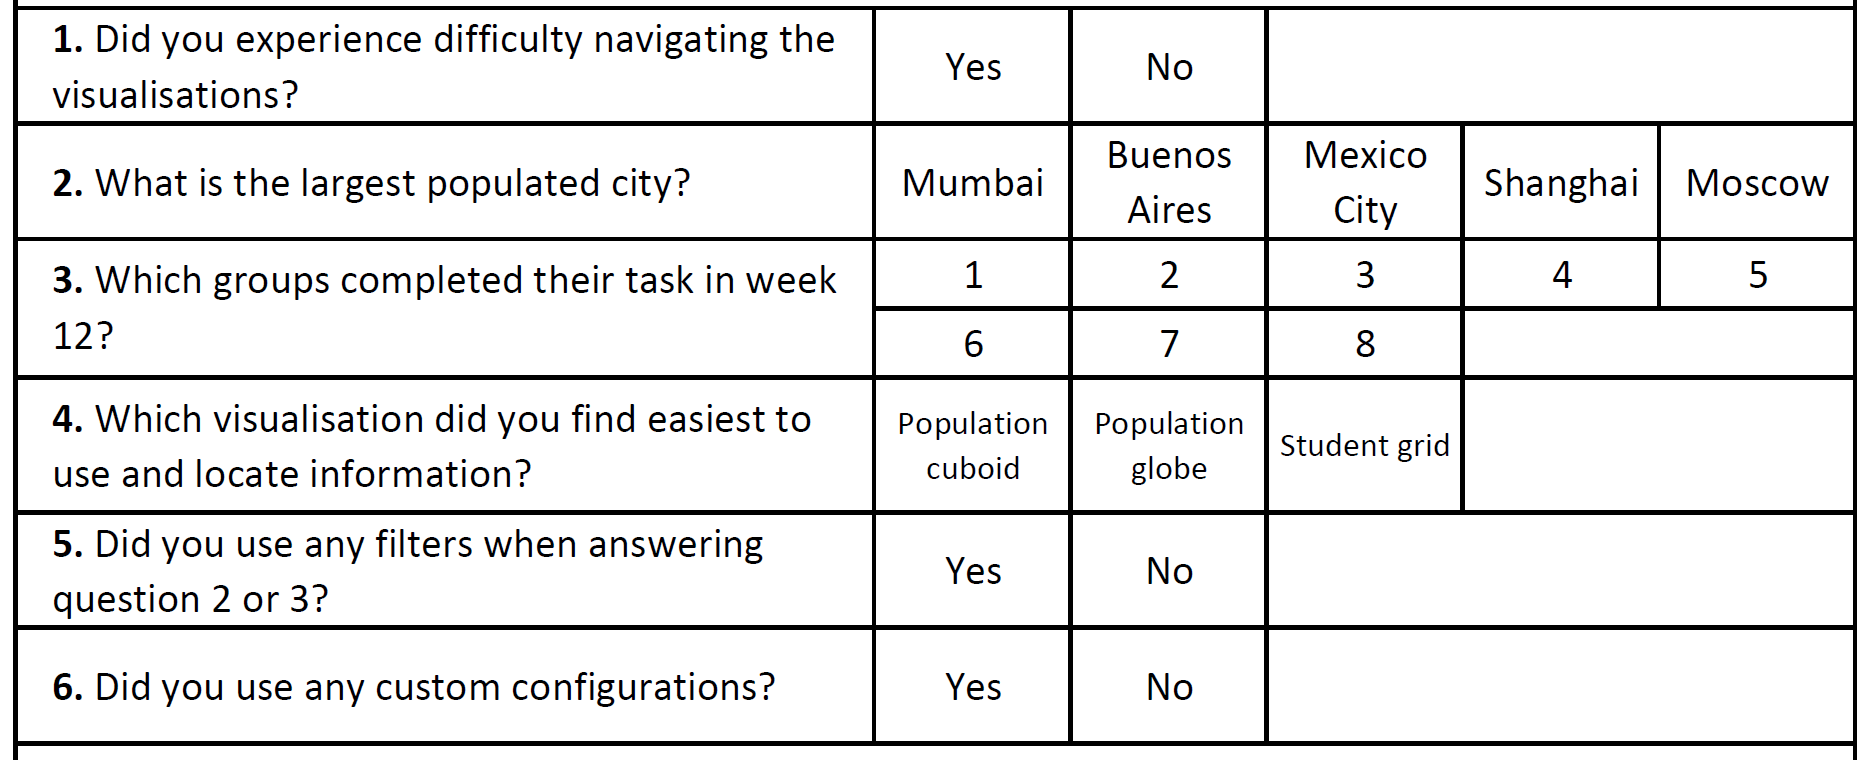
\includegraphics[width=\textwidth]{images/design/questionnaire}

	% }

}

\chapter{Testing} {

	\section{Mocha asynchronous support} {
	\label{app:mocha_asynchronous_support}
		%!TEX root = ../../../report.tex

\begin{figure}[H]
	\newcommand{\basicstyle}{\scriptsize}
    \captionsetup[subfigure]{aboveskip=0em,belowskip=-0.2em}
	\begin{subfigure}[b]{0.45\textwidth}
        %!TEX root = ../../../report.tex

\begin{lstlisting}[basicstyle=\basicstyle]
	doSomethingAsync()
		.then(function (result) {
			result.should.equal('foo');
			done();
		}
	);
\end{lstlisting}

        \caption{Callback}
        \label{fig:mocha_callback}
    \end{subfigure}
    \begin{subfigure}[b]{0.55\textwidth}
		%!TEX root = ../../../report.tex

\begin{lstlisting}[basicstyle=\basicstyle]
	return doSomethingAsync()
		.then(function (result) {
			// Return the result from the promise.
			return result.should.equal('foo');
		}
	);
\end{lstlisting}

        \caption{Promise}
        \label{fig:mocha_promise}
    \end{subfigure}
	\caption{Mocha asynchronous support.}
	\label{fig:mocha_asynchronous_support}
\end{figure}

	}

	\section{Chai as Promised} {
	\label{app:chai_as_promised}
		%!TEX root = ../../../report.tex

\begin{figure}[H]
	\centering
	\begin{lstlisting}
		return doSomethingAsync().should.eventually.equal('foo');
	\end{lstlisting}
	\caption[Chai as Promised]{Chai as Promised.}
    \label{fig:chai_as_promised}
\end{figure}

	}

	\section{Mocha structure} {
	\label{app:mocha_structure}
		%!TEX root = ../../../report.tex

\begin{lstlisting}
	describe('Array', function() {
		describe('#indexOf()', function() {
			it('should return -1 when the value is not present', function() {
				expect([1,2,3].indexOf(5)).to.equal(-1);
			});
		});
	});
\end{lstlisting}

	}

	\section{Mocha hooks} {
	\label{app:mocha_hooks}
		\begin{figure}[H]
	\centering
	\begin{lstlisting}
		describe('hooks', function () {

			before(function () {
				// runs before all tests in this block
			});

			after(function () {
				// runs after all tests in this block
			});

			beforeEach(function () {
				// runs before each test in this block
			});

			afterEach(function () {
				// runs after each test in this block
			});

			// test cases

		});
	\end{lstlisting}
	\caption[Mocha hooks]{Mocha hooks.}
	\label{fig:mocha_hooks}
\end{figure}

	}

	\section{Testing style} {
	\label{app:testing_style}
		%!TEX root = ../../report.tex

\begin{figure}[H]
	\centering
	%!TEX root = ../../report.tex

\begin{figure}[H]
	\centering
	%!TEX root = ../../report.tex

\begin{figure}[H]
	\centering
	\input{code/testing/style}
	\caption[Testing style]{Testing style.}
	\label{fig:testing_style}
\end{figure}

	\caption[Testing style]{Testing style.}
	\label{fig:testing_style}
\end{figure}

	\caption[Testing style]{Testing style.}
	\label{fig:testing_style}
\end{figure}

	}
	
}